\documentclass[tikz]{standalone}
\usepackage{tikz}
\usetikzlibrary{positioning, graphs}
\usetikzlibrary{graphs.standard}
\usetikzlibrary{arrows.meta}
\begin{document}
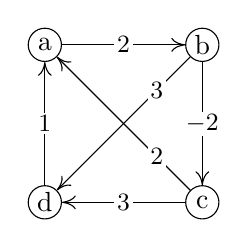
\begin{tikzpicture}
\begin{scope}
		[vertex/.style={draw,circle,inner sep = 0em, minimum size = 1.2em},
		 edgelabel/.style = {fill = white, inner sep = 0.1em, font=\small}]
		\node[vertex] (a) at (0,0) {a};
		\node[vertex] (b) at (2,0) {b};
		\node[vertex] (c) at (2,-2) {c};
		\node[vertex] (d) at (0,-2) {d};
		
		\draw[-{>[length=5, width=5]}] (a) to node[edgelabel] {$2$} (b);
		\draw[-{>[length=5, width=5]}] (b) to node[edgelabel] {$-2$} (c);
		\draw[-{>[length=5, width=5]}] (b) to node[edgelabel, near start] {$3$} (d);
		\draw[-{>[length=5, width=5]}] (c) to node[edgelabel, near start] {$2$} (a);
		\draw[-{>[length=5, width=5]}] (c) to node[edgelabel] {$3$} (d);
		\draw[-{>[length=5, width=5]}] (d) to node[edgelabel] {$1$} (a);
\end{scope}
\end{tikzpicture}
\end{document}